\documentclass[12pt,a4paper,final,oneside,openany]{memoir}

\usepackage[titelside, en, nat]{ku-forside}
\usepackage[english]{babel}
\usepackage[utf8]{inputenc}
\usepackage[T1]{fontenc}
\usepackage[british]{isodate}
\usepackage{booktabs}
\usepackage{fixltx2e}
\usepackage{nameref}
\usepackage{amsmath}
\usepackage{mathtools}
\usepackage[lofdepth,lotdepth]{subfig}
\usepackage{multirow}
\usepackage{float}
\usepackage{hyperref}
\usepackage{color}
\usepackage{xcolor}
\usepackage{cite}
\usepackage{url}
\usepackage[verbose]{wrapfig}
\usepackage[ruled,vlined]{algorithm2e}
\usepackage{multirow}
\usepackage{booktabs}
\usepackage{array}
\usepackage{footnote}
\usepackage{amsthm}
\usepackage{lettrine}

\newtheorem{theorem}{Theorem}

\theoremstyle{definition}
\newtheorem{definition}{Definition}[section]

\def \CodeName{BDOS }
\def \CodeNameFull{BDOS (Big Data Object Store)}

\titel{\CodeName}
\undertitel{A semantics aware big data object-based storage system}
\forfatter{Steffen Karlsson -- \texttt{ckh340@alumni.ku.dk}}
\opgave{Master's Thesis}
\dato{August 2016}
\vejleder{\textbf{Supervisor:} Professor Brian Vinter}

\renewcommand*{\cftpartname}{Part\space}
\cftpagenumbersoff{part}

\newcommand{\subimgwidth}{.5\textwidth}
\newcommand{\imgwidth}{.8\textwidth}

\def\thefigure{\arabic{figure}}
\setcounter{tocdepth}{1}

\renewcommand{\LettrineFontHook}{\sffamily}
\newcommand{\firstletter}[1]{\lettrine[lines=2, loversize=0.2, findent=0.4em]{\textbf{#1}}}

\newcommand{\todo}[1]{{\color{red} \textbf{TODO:}} #1}

\newcommand{\etal}{\textit{et al}. }
\newcommand{\ie}{\textit{i}.\textit{e}., }
\newcommand{\eg}{\textit{e}.\textit{g}. }

\usepackage{tikz, blindtext}
\makechapterstyle{box}{
  \renewcommand*{\printchaptername}{}
  \renewcommand*{\chapnumfont}{\normalfont\sffamily\huge\bfseries}
  \renewcommand*{\printchapternum}{
    \flushright
    
\begin{tikzpicture}
      \draw[fill,color=black] (0,0) rectangle (1.5cm,1.5cm);
      \draw[color=white] (0.75cm,0.75cm) node { \chapnumfont\thechapter };
    \end{tikzpicture}
  }
  \renewcommand*{\chaptitlefont}{\normalfont\sffamily\Huge\bfseries}
  \renewcommand*{\printchaptertitle}[1]{\flushright\chaptitlefont##1}
}

\renewcommand*{\chaptitlefont}{\normalfont\sffamily\Huge\bfseries}

\makepagestyle{diku}
\makeevenhead{diku}{\sffamily\rightmark}{}{}
\makeoddhead{diku}{\sffamily\rightmark}{}{\sffamily\currenttitle}
\makeevenfoot{diku}{}{\sffamily\thepage}{}
\makeoddfoot{diku}{}{\sffamily\thepage}{}
\makeheadrule{diku}{\textwidth}{1pt}
\makeheadposition{diku}{flushright}{flushright}{}{}   

\begin{document}
\pagestyle{plain}
\frontmatter
\clearpage
\maketitle

\vspace{3cm}
\addcontentsline{toc}{chapter}{Abstract}
\begin{abstract}
The goal of the project is to design and implemented a file archive for big data analysis with high performance and scientific data in mind. Existing MapReduce\cite{Dean:2008:MSD:1327452.1327492} frameworks such as the commonly used Apache Hadoop\cite{PageHadoop} is designed and developed for different purposes than what they are used for nowadays. 

The conventional file system approach with fixed size data blocks implemented in Hadoop makes it suboptimal for scientific data processing because splitting data at arbitrary positions means that high-level data structures such as NetCDF data and multidimensional arrays are distributed across multiple machines. A consequence of this is increased latency and intercommunication between machines during data processing.
\newline

Hadoop has previously been investigated and evaluated speci\-fically for scientific data-intensive operations\cite{fadika2012evaluating} and even extended and modified for individual use-case such as NetCDF\cite{buck2011scihadoop}.
\newline

This project introduces \CodeNameShort, a distributed semantic oriented file archive for big data analysis that preserves the structure of data by jointly storing semantically coherent data parts of arbitrary size. The responsibility of correctly splitting the data is transitioned towards the end-user and thus not inaccurately made by the system. The system will be targeted inexpensive commodity hardware like other similar frameworks and will thus primarily rely on the underlying file system for redundancy and hardware for recovery.
\newline

The \CodeName framework provides a range of different system customizations and data related opportunities such as instance based virtualization and the unique and innovative opportunity of virtual replication at a data level specified independently for each entry, 	instead of at a machine level. The framework provides a public available core API that exposes a vast amount of high level routines for developing powerful and useful extensions and applications. The project introduces such an extension BDAE (\textit{/b'dei'/}) which models the notion of a data access and processing layer for \CodeNameShort.

\end{abstract}

\setlength{\cftpartnumwidth}{4em}

\chapter{Preface}

\clearpage
\tableofcontents*

%\clearpage
%\listoffigures*

\mainmatter
\chapterstyle{box}
\pagestyle{diku}

\counterwithout{table}{chapter}
\counterwithout{figure}{chapter}
\BigLetter{A}{ progressively} increasing challenge in high performance computing (HPC) is how to store the large amount of data on disk efficiently, especially with the ubiquitous enthusiasm for Big Data Analysis (BDA) frameworks, within the area of influence. A commonly used distributed computation framework for BDA is Apache's Hadoop\cite{PageHadoop}, where data access is based on the Hadoop Distributed File System (HDFS) \cite{Shvachko:2010:HDF:1913798.1914427} and the primary execution model is based on MapReduce\cite{Dean:2008:MSD:1327452.1327492}. These frameworks are developed under different circumstances, and with different purposes compared to what they are presently used.
\newline

HDFS, as well as the Google File System \cite{Ghemawat:2003:GFS:945445.945450}, follows a centralized architectural master/slave organization (described in \cite{Tanenbaum:2006:DSP:1202502} and briefly in \cite{Wilkinson:1998:PPT:289352}) where what is denoted as NameNode acts as the master. This server maintains attributes such as permissions and namespace tree for slaves. Also, it implements a proxy to handle operations realised on the file system at the slaves. 
\newline

Writing to the Hadoop file system can likely cause what's known as the data residual problem (Figure \ref{fig:data-residual}). Thus, semantically correlated or coherent data can be distributed across different servers. Hadoop is implemented using a conventional file system approach, \ie fixed sized blocks of 64MB. 
\newpage

\begin{figure}
	\centering
	\hspace*{15mm}
	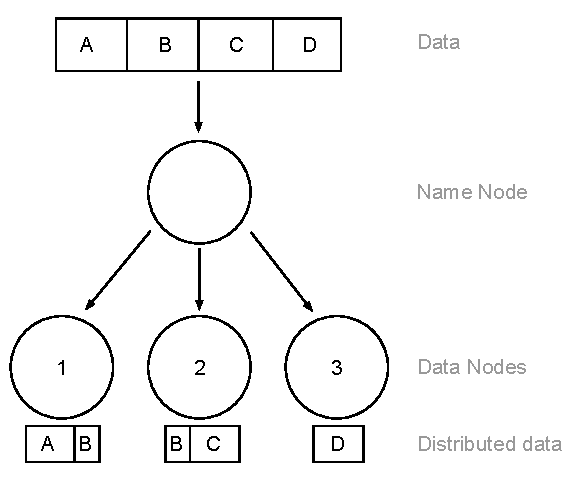
\includegraphics[scale=0.8]{pdf/data-residual.pdf}
	\caption[HDFS data residual problem]{HDFS data residual problem which ultimately requires Data Node 1 and 2 to exchange data for a consistent processing of block B, leading to an increased I/O cost. \label{fig:data-residual}}
\end{figure}

As a matter of fact, the only case where data partitioning is ensured to be avoided is when the \textit{size of the data} modulo \textit{the block size} is equal to zero. As a consequence, individual computer scientist are required to implement a network communication protocol between the slaves to handle this problem, which typically causes increased latency. The goal is to ensure a consistent view and process of the coherent data representations.

\section{Problem definition} \label{sec:problem}
\begin{quotation}
\hspace*{-7mm}
\textit{Firstly, analyze and investigate whether a distributed parallel file system that efficiently hides latency and reduce IO-cost is feasible. Secondly, if such a system is feasible implement a prototype in a sensibly selected language, architecture and environment.} \newline
\end{quotation}

\section{Related work} \label{sec:related}
Existing implementations and research projects within the field of big data analysis frameworks and distributed parallel file systems relevant to this project will be described in this section, including the once previously mentioned.

\subsection*{Hadoop}
Hadoop was originally described in 2010 by Shvachko \etal \cite{Shvachko:2010:HDF:1913798.1914427}. The Apache and Yahoo! developed framework is designed to store and analyze enormous datasets. It provides the distributed hierarchical file system with directories and archives HDFS, as data access layer (DAL) and a primary execution model based on the programming paradigm MapReduce (sharing this feature with the following computing platform), outlined in Definition \ref{def:mapreduce}.
\vspace*{2mm}

\begin{definition}[MapReduce] \label{def:mapreduce}
\textit{A programming paradigm and an associated implementation presented by Dean and Ghemawat} \cite{Dean:2008:MSD:1327452.1327492} \textit{used for data generation, analysis and processing. Fundamentally it is assembled by two separate user specified functions:} \texttt{map} \textit{and} \texttt{reduce}\textit{, which at execution time are parallelized automatically.}
\end{definition}
\vspace*{2mm}

HDFS implements a master/slave architecture where the NameNode server acts as the master and the DataNodes are the slaves. Metadata and application data are stored separately on respectively master and slave. Having a stateful master without replication is a single point of failure  as described by Yahoo! in the Hadoop developer tutorial:

\begin{quotation}
	\textit{"The single point of failure in a Hadoop cluster is the NameNode $\ldots$ loss results in cluster unavailability. The permanent loss of NameNode data would render the cluster's HDFS inoperable."}\cite{YahooDocumentation}
\end{quotation}

Additionally it's a potential bottleneck in a system, but in this project it's a tradeoff between throughput and accessibility.

\subsection*{Facebook (Hadoop)}
Approximately 40\% percentage of all incidents at the Facebook Data Warehouse is somewhat Hadoop related (Figure \ref{fig:fb-hadoop-incidents}), many of those is due to the single point of failure (SPOF) error at the NameNode, which causes more or less the whole Hadoop cluster to be unavailable and thus not correctly functioning. Improving HDFS and SPOF error at the NameNode is therefor an essential task to ensure that the ecosystem are efficient and reliable.

\begin{figure}[h!]
	\centering
	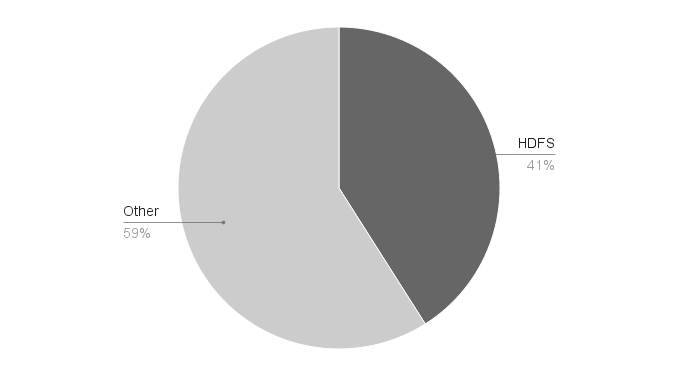
\includegraphics[scale=0.48]{img/fb-hadoop-incidents.png}
	\caption[Incidents at Facebooks Data Warehouse]{Incidents at Facebooks Data Warehouse by percentage at the responsible part, others including user specified jobs etc.\cite{FacebookHadoopImprovement}. \label{fig:fb-hadoop-incidents}}
\end{figure}

\newpage
Facebooks engineers designed a solution based on a so-called Avatar\-node, as a functioning hot fail-over solution, turning the existing NameNode into a highly-available server. The open source Avatarnode is essentially two NameNodes wrapped in an Apache ZooKeeper\footnote{Apache ZooKeeper\cite{PageZookeper} is a centralized service provider for configuration information and naming etc.} instance, with support for manual failover. The two NameNode instances behave as an active one and a standby with internal virtual IP address (VIP), handled by ZooKeeper, \ie each client request is initialized through that to get the VIP of the primary node (Figure \ref{fig:facebook-avatarnode}).
\newline

Synchronization between the active and the standby NameNode instance is managed by a NFS (Network File Server).
\vspace*{3mm}

\begin{figure}[h!]
	\centering
	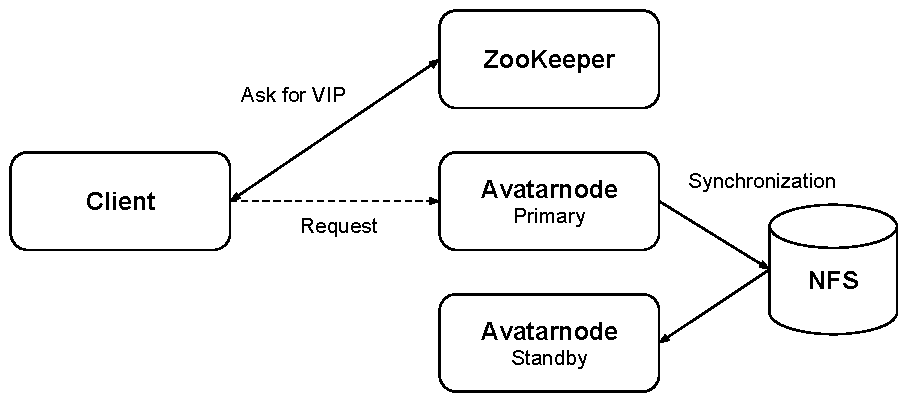
\includegraphics[scale=0.8]{pdf/facebook-avatarnode.pdf}
	\caption[Avatarnode: Facebooks Hadoop implementation]{Control flow of the AvatarNode and ZooKeeper with virtual IP address and network file server for synchronization. \label{fig:facebook-avatarnode}}
	\vspace*{3mm}
\end{figure}

Facebook claims that the solution leads to a projected result of 50\% lesser planned downtime, \ie a critical time where that part of the warehouse is unavailable. Though, one could certainly come up with new issues arising in this solution:
\begin{itemize}
	\item SPOF error reliability of the Apache ZooKeeper instance, since that is the only access-point now.
	\item SPOF error reliability of the NFS.
\end{itemize}

\subsection*{Hadoop 2.x}
Apache later released in Hadoop \textbf{2.x} \cite{Hadoop2xDocumentation} their solution to the single point of failure problem which they have described as: 

\begin{quotation}
	\textit{"$\ldots$ if that machine or process became unavailable, the cluster as a whole would be unavailable until the NameNode was either restarted or brought up on a separate machine"}. 
\end{quotation}

The solution is based on redundant duplication of the NameNode, such that one machine acts as the active one serving clients and another as the full redundant standby, which allows a fast fail-over in the case that the Active one crashes. The synchronization of logs and state between the two masters can be accomplished in two different ways:
\vspace*{3mm}

\begin{enumerate}
	\item Having at least 3 or more relatively lightweight Quorum Journal Manager (QJM) daemons to tolerate the failure of a single machine, because each modification has to be written to a quorum based majority of the daemons
	
	Major problems in this solution are:
\begin{itemize}
	\item Synchronization (the communication or latency cost of it).
	\item Considerable increase in hardware\footnote{One new machine for the standby and presumably three for the QJMs.}.
\end{itemize}
	\vspace*{3mm}
	
	\item Another option is to use a shared network file server (NFS) storage (Figure \ref{fig:hadoop-2x-nfs}).
	\begin{figure}[h!]
		\centering
		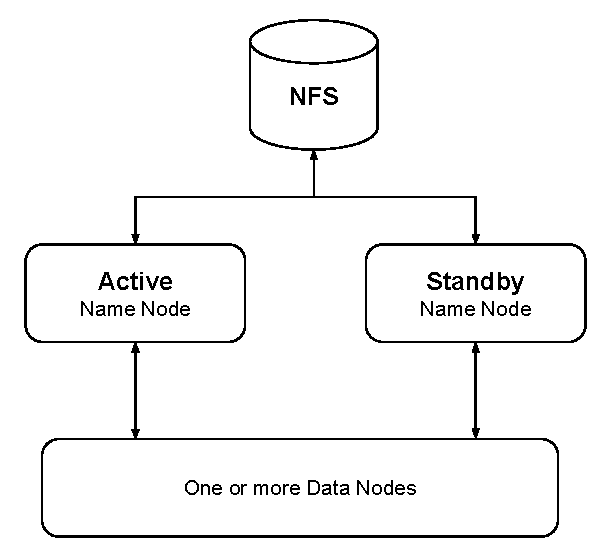
\includegraphics[scale=0.6]{pdf/hadoop-2x-nfs.pdf}
		\caption[Hadoop 2.x NFS solution]{Component diagram of the Hadoop 2.x NFS solution. \label{fig:hadoop-2x-nfs}}
	\end{figure}	

	This approach will undeniably mask the single point of failure (SPOF) error on the NameNode master by the cost and reliability to handle SPOF errors on the network file system abstraction, which in fact in most cases is a single server.
\end{enumerate}

\subsection*{Disco}
Mundkur \etal at Nokia Research Center published in 2011 a paper on their implementation of the distributed computing platform Disco\cite{PageDisco}\cite{Mundkur:2011:DCP:2034654.2034670}. Disco is an easy customizable MapReduce (Defintion \ref{def:mapreduce}) framework with regards to environment and requirements, designed for clusters of commodity server machines. Disco is likewise based on the master/slave architecture and relies on a standard file system and thus, deprioritizes persistent fault tolerance, achievable by a dedicated custom implementation. 
\newline

The single master pattern is as mentioned a single point of failure but is preferred due to consistency over availability (CAP theorem is outlined in \ref{def:cap}).
\vspace*{2mm}

\begin{definition}[CAP Theorem] \label{def:cap}
\textit{Eric Brewer presented in his keynote speech}\cite{Brewer2000} \textit{the CAP (Consistency, Availability, and Partition Tolerance) theorem that states, a distributed system (set of independent computers working together) only at any point in time can guarantee two of the three listed acronym properties, as illustrated in Figure \ref{fig:cap}.}

\begin{figure}[h!]
	\centering
	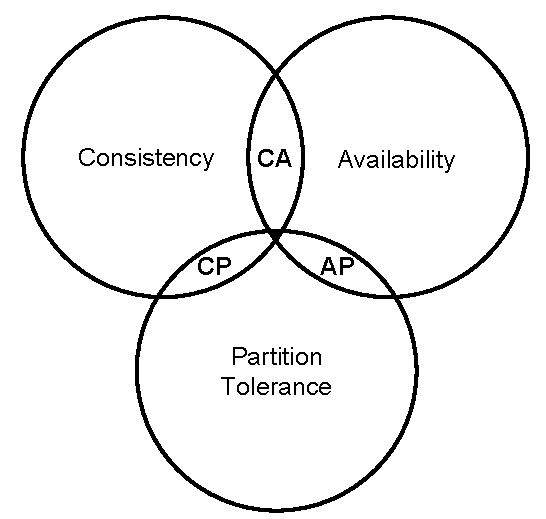
\includegraphics[scale=0.7]{pdf/cap.pdf}
	\caption{Illustrating the concept and limitations of CAP. \label{fig:cap}}
\end{figure}	
\end{definition}

\subsection*{Dynamo}
Dynamo is a highly available key-value storage system presented by Amazon engineers \cite{DeCandia:2007:DAH:1294261.1294281}. The system is implemented using an eventual consistency protocol and thereby sacrifices it under certain scenarios, by cause of availability. 

The reason for this choice is the \textit{"always-on"} user experience on core services on the Amazon platform that Dynamo is used to function. Dynamo uses consistent hashing (Definition \ref{def:ch}) to partition the key space across all available machines. A uniform distribution ultimately leads to a uniform load, assuming the key space access is not too skewed.
\vspace*{3mm}

\begin{definition}[Consitent hashing] \label{def:ch}
\textit{Engineer at Apache, White, describes in his blog post} \cite{PageWhiteCH} \textit{the purpose and demand for consistent hashing. It arose from the problems and limitations experienced with a naive hash-based key space distribution in a distributed system, where adding and removing machines in the network can be a catastrophe from a network bandwidth point of view, due to redistribution of the key space. In consistent hashing, only a fair share proportion from each of the machines is reassigned, while adding or removing machines.}
\end{definition}

\subsection*{Google File System}
Ghemawat \etal at Google describes the scalable distributed file system (GFS: Google File System) designed at implemented for primary developed for internal usage \cite{Ghemawat:2003:GFS:945445.945450}. 

The file system is designed to run on inexpensive commodity hardware like Dynamo and to provide fault tolerance. The architecture is a single stateful master and slave(s) organization, where the (GFS) master maintains all metadata file in the system. 
\newline

A vastly simplified design and sophisticated placement of data on the slaves, together with a strong recovery protocol has been prioritized compared to the risk of a single master (as previously explained). Communication between clients and the master are also widely reduced, by caching slave metadata for further intercommunication on the client eliminating the bottleneck effect on the master.
\vspace*{3mm}

\begin{definition}[Bottleneck effect] \label{def:bottle}
\textit{A part of a system is defined as a bottleneck if it critically limits the remaining system. This component usually has the lowest throughput of all.}
\end{definition}

\section{Proposal} \label{sec:proposal}
The knowledge, features, and compromises in the papers discussed and described in Related work provides the foundation for the research in the project. The ambition of the research is to first of all design a prototype of an alternative to the existing file archives used in big data analysis and secondly if possible to implement it.
\newline

The design of the architectural organization of the prototype is intended to eliminate the complications and issues in the existing solutions that has been described. A desired outcome is a substitute system eliminating data residuals with reduced I/O-cost and complexity and increased performance.
\newline

This can be achieved by splitting data semantically coherent at key positions by the file system, thus, data will be divided into arbitrarily sized chunks instead of fixed. Main challenges includes:
\vspace*{2mm}
\begin{itemize}
	\item Describing a domain specific model to characterize the data semantics.
	\item Defining a direct data mapping for storing and retrieval.
	\item Designing a system that scales as the data and request rate grows, \ie provides consistent and intelligent load balancing.
\end{itemize}

A feasible solution to reduce I/O-cost includes the mechanism of data cleaning, which is an important preprocessing step in big data analysis where \ie following actions can be performed:
\begin{itemize}
	\item Reformatting multidimensional scientific dataset such that identical features are grouped.
	\item Reducing noise.
	\item Transformation and dimensionality reduction (remove redundancy).
\end{itemize}
\vspace*{5mm}

The system seeks to perform the actions as mentioned above in real time since they are computationally simple on modern high-end processors and are attractive to perform before writing data to disk. 
\newline

Furthermore, a straightforward extension is to measure and store elemental statistics per dataset in a fashionable and state-of-the-art way. It is ultimately an ambition to integrate the same execution model as in \eg Hadoop and Disco, namely MapReduce around the implemented file archive to compose a full big data analysis framework alternative.

\section{Assumptions} \label{sec:assumption}
Following assumptions are constructed first and foremost to limit the prototype to the field of study relevant for this project and secondly to match the surrounding environment and settings.

\begin{itemize}
	\item The solution is targeted research and scientific datasets. 
	\item The solution is targeted and used for big data analysis.
	\item A full dataset is accessed, processed or modified at once.
	\item Individual data entries can be processed and analyzed independently and the order of data entries is irrelevant.
	\item The majority of the datasets are passive, \eg not quite accessed as much as expected in systems like GFS.
\end{itemize}

\section{Outline}
Part \ref{prt:sofa} explains the needs and requirements of the file archive for big data analysis based on the knowledge learned from analysis existing solutions in Chapter \ref{sec:introduction}. Additionally, it describes the architecture and design along with the implementation of the prototype. Part \ref{prt:extensions} explains the implementation of an extension build on top of the file archive based on the API described in Chapter \ref{chp:api}. Part \ref{prt:evaluation} finally, validates the correctness and measures the efficiency of the final solutions in addition to describing the plans for the future.

%\part{Big Data Area Network} \label{part:bdan}
%\BigLetter{D}{efining} and designing a distributed system used as a file archive is a compromising process of electing architecture, communication and security among others. This chapter describes and discusses the choices and opportunities regarding what henceforward will be denoted as \CodeNameFull. 

\begin{figure}
	\centering
	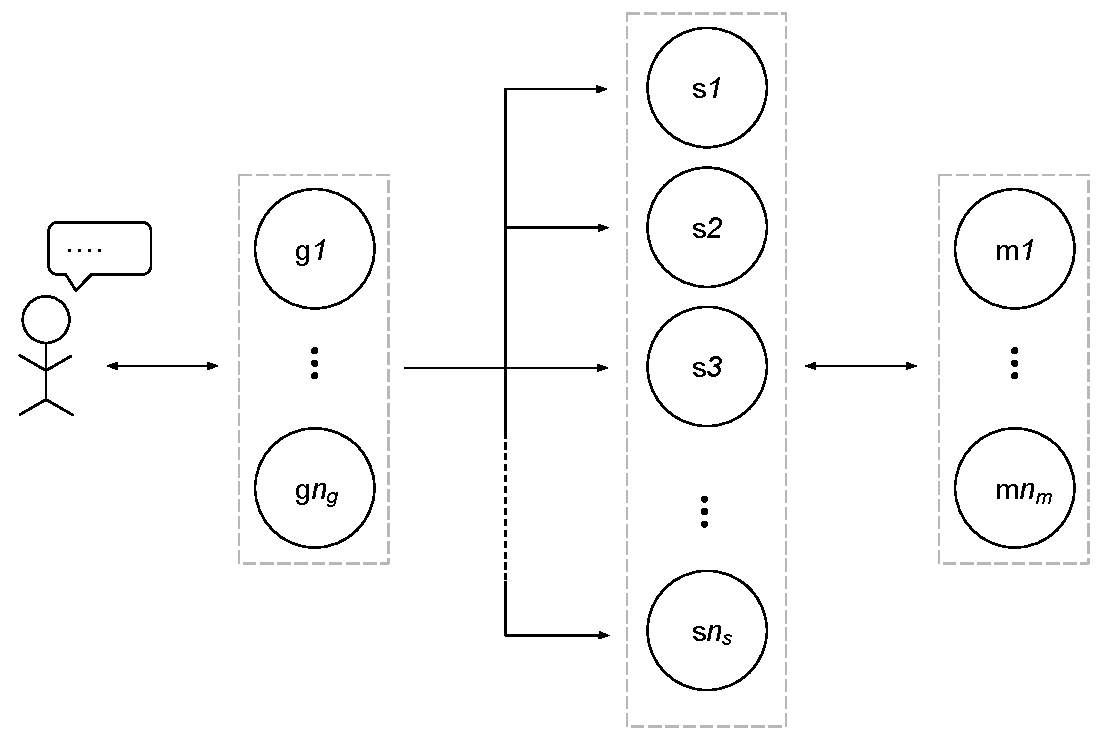
\includegraphics[scale=0.60]{pdf/sofa-overview.pdf}
	\caption[General overview of \CodeName]{General overview of \CodeName and the participating components and their associates, including $n_g$ gateways denoted by $\text{g}1 \ldots \text{g}n_g$, $n_s$ storage nodes by $\text{s}1 \ldots \text{s}n_s$ and $n_m$ monitors by $\text{m}1 \ldots \text{m}n_m$. \label{fig:sofa-overview}}
\end{figure}

\section{Overview}
This project is an alternative to the existing file archives targeting big data analysis frameworks; the architectural structure will be influenced and inspired by those described in related work (Section \ref{sec:related}), both by characteristics and feature, but certainly from inaccuracies too. 
\newline

The architecture of the file archive seeks to model an interpretation of a storage area network (SAN) primarily used for research and scientific related big data analysis, operating in a trusted homogeneous computing environment. The illustration at Figure \ref{fig:sofa-overview} depicts the general overview and flow of the system just described, where each component is examined subsequently in Chapter \ref{chp:components}.

\section{Hardware} \label{sec:hardware}
The framework is designed first and foremost to execute on a homogeneous collection of machines connected to a network such as a cluster, but the choice could have been a grid (a collection of heterogeneous machines) too. 
\newline

The implementation will be targeted inexpensive commodity hardware like Dynamo or the Google File System (Section \ref{sec:related}) and will be assembled by JBODs (Defintion \ref{def:jbod}) for this first version.

\vspace*{3mm}
\begin{definition}[JBOD] \label{def:jbod}
\textit{It is an acronym for Just a Bunch of Disks and is a hardware architecture with multiple hard drives, but without configuration of RAID and thus doesn't provide redundancy nor performance improvements.}
\end{definition}

The fact that the underlying component is a file archive related system built by bricks (Definition \ref{def:brick}) make clusters an obvious choice for a prototype.

\vspace*{3mm}
\begin{definition}[Brick] \label{def:brick}
\textit{A brick is defined as a component of a homogeneous distributed system, where each of them is functional equivalent and are contributing uniformly and have equal rights.}
\end{definition}
\vspace*{3mm}

\section{Architectural style} \label{sec:architectural-style}
The overall architecture of the project will be affected by knowledge and benefits from existing solutions (Section \ref{sec:related}) along with the theoretical background knowledge acquired by Tanenbaum \etal's description of distributed system architectures\cite{Tanenbaum:2006:DSP:1202502}. 
\newline

The result will seek to model the notion of a hybrid related distributed system with a decentralized collection of interconnected peer-to-peer storage nodes accessible by potentially multiple replicated stateless gateway servers and observed by one or more monitors.

\begin{figure}[h!]
	\centering
	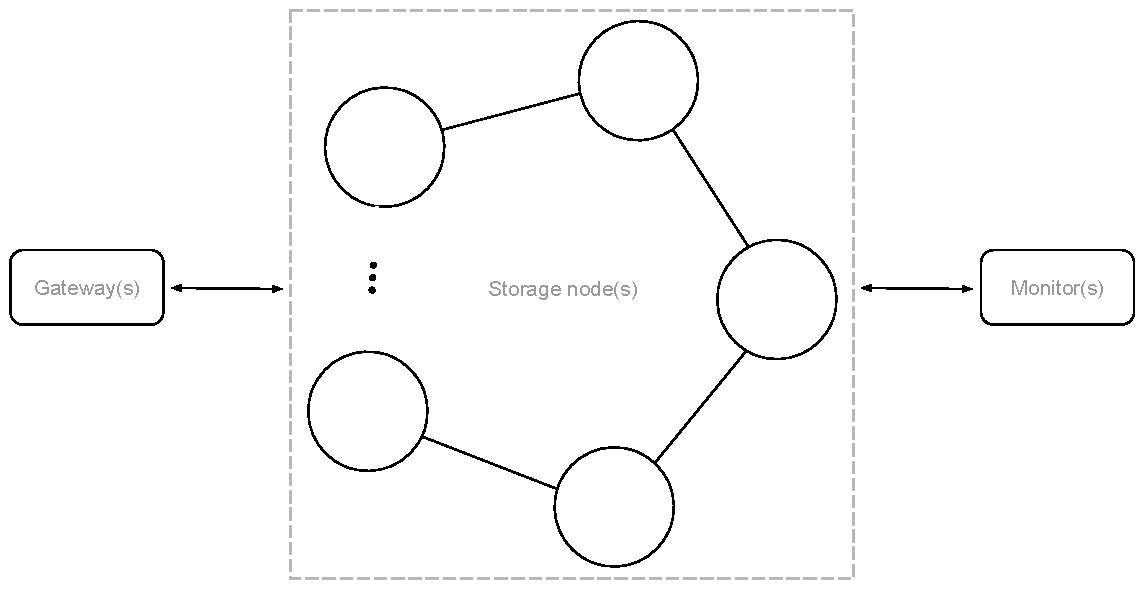
\includegraphics[scale=0.7]{pdf/architecture-overview.pdf}
	\caption[Architectural overview]{Architectural overview of the hybrid related distributed system reflecting a zero-hop distributed hash table ring of storage nodes. \label{fig:architecture-overview}}
\end{figure}

The architecture of the interconnected storage nodes (Figure \ref{fig:architecture-overview}) is highly influenced by Dynamo and will reflect a zero-hop distributed hash table (Definition \ref{def:dht}) and thus provides full data consistency concerning the CAP theorem (Definition \ref{def:cap}). Unfortunately, this also means that complexity regarding the consistency protocol increases at a membership protocol level.
\newline

The design and structure of the storage node will be described as part of Chapter \ref{chp:nodes} in Section \ref{sec:storage}, the gateway in Section \ref{sec:gateway} and the monitor in Section \ref{sec:monitor}.
\newpage

\begin{definition}[Distributed Hash Table] \label{def:dht}
\textit{DHT is undoubtedly the most-used organized peer-to-peer overlay network infrastructure, a procedure to arrange processes/nodes and links between them. Each node is assigned a unique identifier and a sub key-space\footnote{The available identifiers between two neighbor nodes}  generated by special hash-function, defined for that particular system and thereby placed onto the ring. Figure \ref{fig:dht} illustrates an example of a DHT ring.}

\begin{figure}[h!]
	\centering
	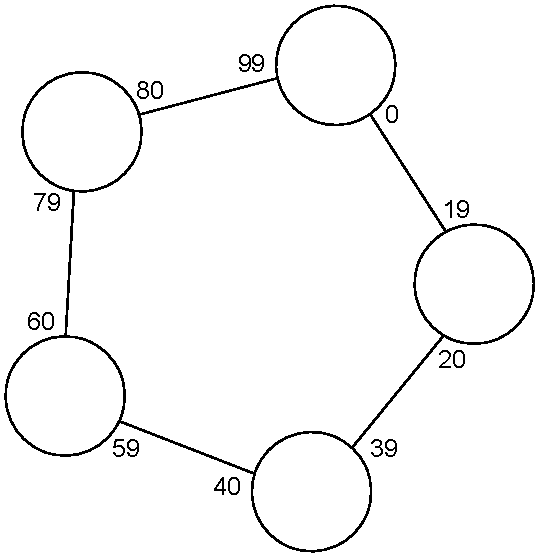
\includegraphics[scale=0.6]{pdf/dht.pdf}
	\vspace*{3mm}
	\caption[]{Example of a distributed hash table example with a key-space size of 100 and 5 storage nodes available. \label{fig:dht}}
\end{figure}
\end{definition}

\section{Communication} \label{sec:communication}
%TODO 

\section{Partitioning and distribution} \label{sec:pandd}
The partitioning and distribution protocol in \CodeName is based on consistent hashing (\reference{def:ch}{sec:partitioning}) and the round-robin load balancing algorithm (Definition \ref{def:rr}). The downside of this distribution algorithm is that it does not take state, availability and workload among other properties of the servers into account. 
\newline

However, this should be adequate assuming data is large enough and the framework primarily is expected to be operating in homogeneous and high-performance computing environment like a cluster (Section \ref{sec:presumptions}). Furthermore, one of the assumptions (Section \ref{sec:assumption}) is to implement a transparent but suitable load balancing protocol with big data analysis in mind.
\vspace*{3mm}

\begin{definition}[Round-robin] \label{def:rr}
\textit{A simple, fair share and starvation free load balancing algorithm that is easy to implement. The algorithm is distributing elements until there are no more among the available servers in a one-by-one or chunk-by-chunk fashion, thus the name of the algorithm.}
\end{definition}
\vspace*{3mm}

\begin{figure}[h!]
	\centering
	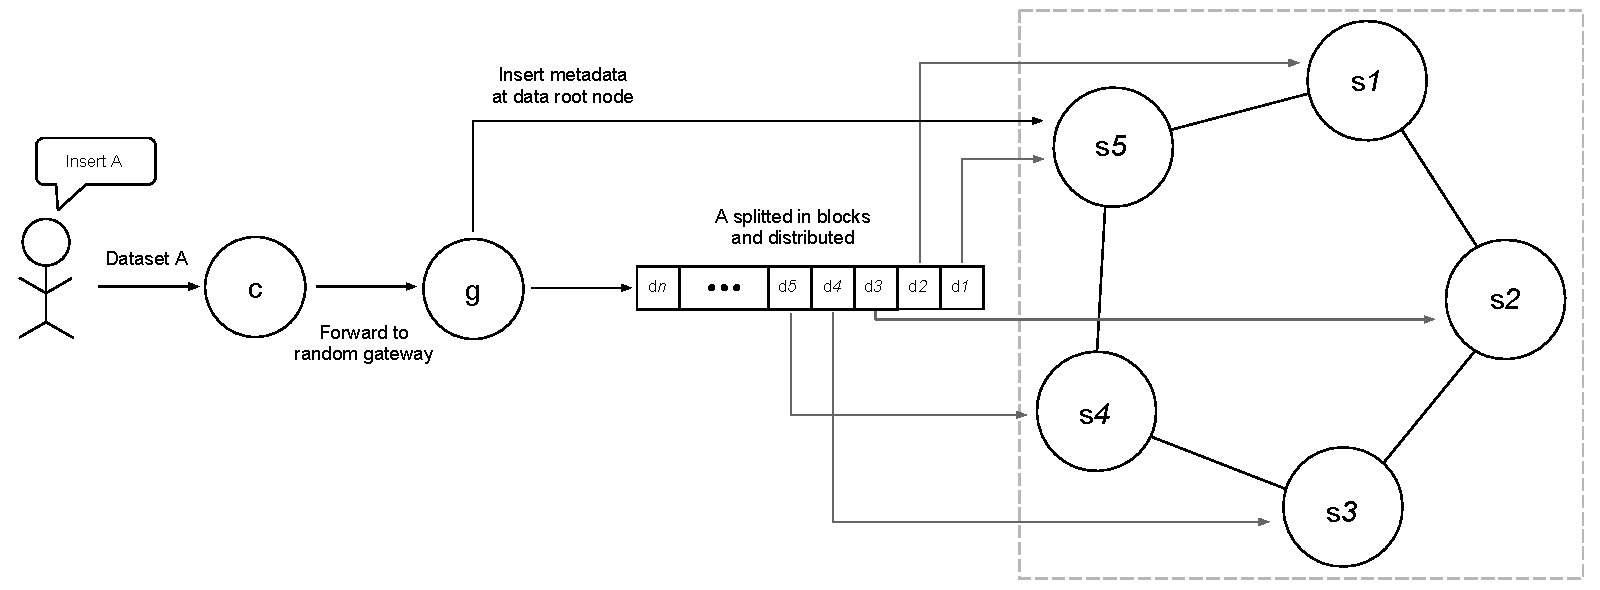
\includegraphics[scale=0.5]{pdf/rr-partitioning.pdf}
	\caption[Overview of the partitioning and data distribution protocol]{General flow of the partitioning and data distribution protocol in \CodeName, assuming one gateway server \textit{g} and a client \textit{c} attempting to insert data \textit{A} consisting of \textit{n} blocks $\text{d}1 \ldots \text{d}n$.\label{fig:rr-partitioning}}
\end{figure}

Figure \ref{fig:rr-partitioning} illustrates the general flow of the preferred partitioning and distribution protocol. The data is distributed from the client to an arbitrary gateway server, where it is assigned a unique identifier using consistent hashing (as in Amazons Dynamo project) and partitioned into approximately\footnote{As described in section \ref{sec:objectives} is one of the ambitions to store arbitrary sized block.} equal block sizes. The blocks are distributed in a round-robin fashion to the storage nodes, after the metadata for the data is assigned to the root server\footnote{The server responsible for the data, which is determined by the identifier.}.

\section{Naming and virtualization} \label{sec:virtualization}
A requirement is that each instance of \CodeNameFull is associated with a specific global instance name (Section \ref{sec:configuration}) \eg based on the research area or even specific data types. This name is predominantly used to virtualize components, data, and caches and thereby supporting multiple executions of \CodeName instances at once, with own domains.
\newline

Elements in the framework are identified using a structured naming based technique\cite{Tanenbaum:2006:DSP:1202502}, where each semicolon denotes an explicit and more specific context. 

\subsubsection*{Nodes}
The pattern of the naming scheme of node components (depicted at as a general overview at Figure \ref{fig:sofa-overview} and described in Chapter \ref{chp:nodes}) are characterized as following:
\begin{equation*}
	\texttt{sofa}:<\text{instance name}>:<\text{type ref}>:<\text{sequence number}>
\end{equation*}
, where \texttt{type ref} is one of following component types: gateway, storage or monitor and the \texttt{sequence number} is a positive increasing number in range $0\ldots n$ where $n$ is either the number of gateways, storage nodes or monitors respectively.

\subsubsection*{Data}
\begin{equation*}
	<\text{instance name}>:<\text{data type}>:<\text{data name}>
\end{equation*}

The naming scheme of data (Chapter \ref{chp:components}) are defined as above, where \texttt{instance name} is the same as above, the \texttt{data type} is an optional parameter if the framework supports multiple types. The name of the data is required to be unique and specified as \texttt{data name}. The \texttt{sofa} identifier is not necessary since the data is only accessible in a sofa based context.

\section{Redundancy and replication}
Redundancy in \CodeName is carried out using \eg software RAID-Z in ZFS (Description \ref{def:zfs}), which provides block-level striping with double distributed parity, that ensures fault tolerance by upto two failed drives. The motivation for this is that the existing replication protocols in \eg Hadoop and Google File System (Section \ref{sec:related} and \ref{sec:replication}) are using a vast amount of space and communication are too expensive considering that the primary usage of this is big datasets.
\newline

If the redundancy protocol however is based on erasure codes then it is no longer replication, but fault tolerance with a degree of durability. This type of responsibility is in this system carried out in hardware by the JBODs, such that there is no need for the extensive amount of network data transfer.

\begin{definition}[ZFS] \label{def:zfs}
\textit{It is composed of one or more virtual storage pools which are a collection of virtual devices that can be interpreted as a RAID (Redundant Array of Independent Disks) set in a standard file system.}
\newline

\textit{ZFS is an extensive 128-bit addressable file system that always is consistent on disk, this is because it performs a copy on write operation when adding new data, \ie writing modified data into a new space and reuse the old space in the future, thus eliminating the write hole error (corrupted file system) \eg on power loss.}
\end{definition}

\section{Recovery} \label{sec:recovery}
The RAID-Z configuration described in the previous section with the purpose of replication are also used as a basic recovery protocol to conceal disk failures. A second recovery initiative is redundant multipaths to efficiently hide server error.
\newline

The system will run on economical low-cost hardware such as JBODs (Definition \ref{def:jbod}) as explained in section \ref{sec:hardware}. Having SAS-controlled\footnote{Serial Attached SCSI: serial point-to-point protocol for moving data} disks enables fail-over features such as multipathing (Definition \ref{def:multipath}) that allows redundant data paths between host servers and the block-level devices.

\begin{figure}[h!]
	\vspace*{3mm}
	\centering
	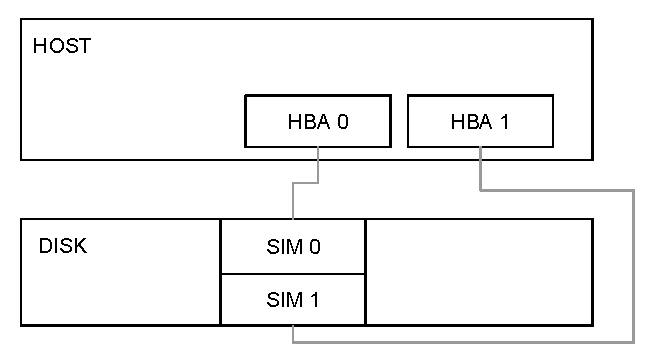
\includegraphics[scale=1]{pdf/1host-1disk.pdf}
	\vspace*{3mm}	
	\caption[Simple JBod setup]{JBod setup with one host and one array of disks.\label{fig:1host-1disk}}
\end{figure}
\newpage

Figure \ref{fig:1host-1disk} illustrates a simple example with one host and one array of disks, where:
\begin{itemize}
	\item \textbf{HBA} (Host Bus Adapter) is the local controller on the computer that connects it to other storage or network devices.
	\item \textbf{SIM} (SAS Interface Module) is the storage device controller.
\end{itemize}

Figure \ref{fig:2host-2disk} includes another more complex example to show the scalability with multiple hosts and disks.
\begin{figure}[h!]
	\centering
	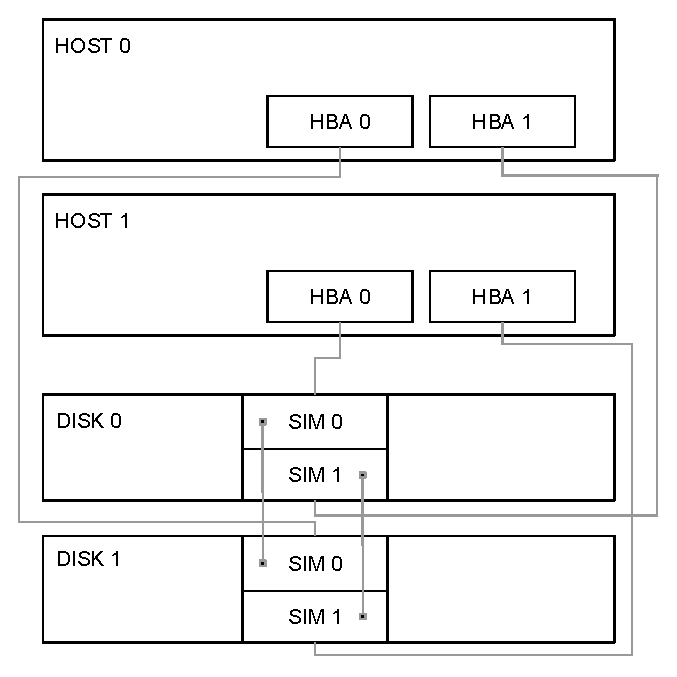
\includegraphics[scale=1]{pdf/2host-2disk.pdf}
	\caption[Complex JBod setup]{JBod setup with multiple hosts and multiple disks. \label{fig:2host-2disk}}
\end{figure}

\begin{definition}[DM Multipath] \label{def:multipath}
\textit{Multipathing is a Linux operating system device mapper for SAS-controlled hard drives that provides I/O fail-over and load balancing, by having numerous paths between host and disk. The configuration of DM Multipath is handled at an operating system level and the device controllers on the storage disks is unaware of such configurations.}
\end{definition}

\section{Security} \label{sec:security}
The focus on data integrity and security have predominantly been given low priority, since the system is expected to execute in a trusted environment, exactly like Amazon Dynamo, thus it is intentionally implemented without internal authentication or authorization.
\newline

Nevertheless, security is evidently an influential component and property at the boundary of the system, one of many actions is \eg using the secure HTTPS connection on the network requests to the entry gateway servers instead of ordinary HTTP. Validation of user input is most certainly also a reasonable action when it comes to security.


%\part{Big Data Context Descriptor} \label{part:bdcd}

%\part{Big Data Query Engine} \label{part:bdqe}

\appendix
%\chapter{Installation Guide} \label{app:installation}
\BigLetter{A}{} installation guide\footnote{Linux-based operation system is preferred} for both \CodeName and BDAE including an available test and example suite with samples such as the ones explained in section \ref{sec:examples} in the analysis phase of \CodeName. The source code archive\footnote{\texttt{<project path>/src/}} of the combined project will onwards be referenced as \texttt{src/} and assumed to be fetched from the repository.

\begin{enumerate}
	\item Install \CodeName:
	
	\begin{lstlisting}[numbers=none, backgroundcolor=\color{sourcebackground}, rulecolor=\color{sourcebackground}, framextopmargin=5pt, framexbottommargin=5pt, frame=tb, xrightmargin=15pt]
	cd src/sofa-project
	bash install.sh
	\end{lstlisting}
	\vspace*{-6mm}
	\item Install BDAE:
	
	\begin{lstlisting}[numbers=none, backgroundcolor=\color{sourcebackground}, rulecolor=\color{sourcebackground}, framextopmargin=5pt, framexbottommargin=5pt, frame=tb, xrightmargin=15pt]
	cd src/bdae-project
	bash install.sh
	\end{lstlisting}
	\vspace*{-6mm}
	\item Create new empty project directory\footnote{Will ahead be denoted as \texttt{example/}}.
	\item Duplicate and modify the system configuration file to fit the purpose:
	
	\begin{lstlisting}[numbers=none, backgroundcolor=\color{sourcebackground}, rulecolor=\color{sourcebackground}, framextopmargin=5pt, framexbottommargin=5pt, frame=tb, xrightmargin=15pt]
	cd example
	cp $SOFA_HOME/sofa/sofa.cfg my_sofa.cfg
	vim my_sofa.cfg
	\end{lstlisting}
	
	\item Enable local SSH\footnote{Extra step on macintosh-based systems available here: \url{http://www.techradar.com/how-to/computing/apple/how-to-enable-ssh-on-your-mac-1305644}} to fully utilize the supplied boot-scripts (explained and exemplified in appendix \ref{app:execution}):
	
	\begin{lstlisting}[numbers=none, backgroundcolor=\color{sourcebackground}, rulecolor=\color{sourcebackground}, framextopmargin=5pt, framexbottommargin=5pt, frame=tb, xrightmargin=15pt, commentstyle=\color{bashcommetcolor}]
	cd ~/.ssh/
	touch authorized_keys
	cat id_rsa.pub > authorized_keys
	
	# Verify by ssh to localhost
	ssh localhost
	\end{lstlisting}
	\vspace*{-6mm}
	\item Install following extra Python 2.7 packages to run all BDAE examples, located in \texttt{\$BDAE\_HOME/examples}:

	\begin{lstlisting}[numbers=none, backgroundcolor=\color{sourcebackground}, rulecolor=\color{sourcebackground}, framextopmargin=5pt, framexbottommargin=5pt, frame=tb, xrightmargin=15pt, commentstyle=\color{bashcommetcolor}, showstringspaces=false]
	# Prerequisite for text.py
	pip install ntlk
	python -c "import nltk; nltk.download('punkt')"
	
	# Prerequisite for avs5m.py
	pip install tifffile
		
	# Prerequisite for NetCDF pop.py
	pip install netCDF4
	\end{lstlisting}
	\vspace*{-6mm}
	\item[$\bullet$] {\sffamily\textbf{NOTE:}} To uninstall \CodeName and BDAE, use following two commands:
	\begin{lstlisting}[numbers=none, backgroundcolor=\color{sourcebackground}, rulecolor=\color{sourcebackground}, framextopmargin=5pt, framexbottommargin=5pt, frame=tb, xrightmargin=15pt, commentstyle=\color{bashcommetcolor}, showstringspaces=false]
	cd src/
	bash clean.sh sofa
	bash clean.sh bdae		
	\end{lstlisting}
\end{enumerate}


\chapter{Execution Guide} \label{app:execution}
{\footnotesize \textit{Assuming the installation guide at appendix \ref{app:installation} is completed.}}
\newline

\BigLetter{A}{} general boot script is provided as part of the installation of \CodeName and can succesfully initialize all three type of server. The script requires that the SSH (explained in appendix \ref{app:installation}) is properly configured on each machine.
\begin{itemize}
	\begin{lstlisting}[numbers=none, backgroundcolor=\color{sourcebackground}, rulecolor=\color{sourcebackground}, framextopmargin=5pt, framexbottommargin=5pt, frame=tb, xrightmargin=15pt, commentstyle=\color{bashcommetcolor}, showstringspaces=false, deletendkeywords={file, list}]
	cd $SOFA_HOME/
	
	# General pattern for the boot script
	bash boot.sh <path to cfg file> <state>
	\end{lstlisting}
	\vspace*{-6mm}

	\item Gateway example:
	\begin{lstlisting}[numbers=none, backgroundcolor=\color{sourcebackground}, rulecolor=\color{sourcebackground}, framextopmargin=5pt, framexbottommargin=5pt, frame=tb, xrightmargin=15pt, commentstyle=\color{bashcommetcolor}, showstringspaces=false]
	bash boot.sh example/my_sofa.cfg gateway storage
	\end{lstlisting}
	\vspace*{-6mm}
	
	\item Storage example:
	\begin{lstlisting}[numbers=none, backgroundcolor=\color{sourcebackground}, rulecolor=\color{sourcebackground}, framextopmargin=5pt, framexbottommargin=5pt, frame=tb, xrightmargin=15pt, commentstyle=\color{bashcommetcolor}, showstringspaces=false]
	bash boot.sh example/my_sofa.cfg storage
	\end{lstlisting}
	\vspace*{-6mm}
	
	\item Monitor example:
	\begin{lstlisting}[numbers=none, backgroundcolor=\color{sourcebackground}, rulecolor=\color{sourcebackground}, framextopmargin=5pt, framexbottommargin=5pt, frame=tb, xrightmargin=15pt, commentstyle=\color{bashcommetcolor}, showstringspaces=false]
	bash boot.sh example/my_sofa.cfg monitor storage gateway
	\end{lstlisting}	
\end{itemize}

Note that the \texttt{state} parameter is a list of node types, where the first element is the kind that the current node will adapt. The rest of the optional element in the list is the kind of nodes that the current one will have an awareness of.
\newline

The nodes are bootable by the python daemon too, in the case of misconfigured SSH or other reasons:
\vspace*{2mm}

\begin{lstlisting}[numbers=none, backgroundcolor=\color{sourcebackground}, rulecolor=\color{sourcebackground}, framextopmargin=5pt, framexbottommargin=5pt, frame=tb, xrightmargin=15pt, commentstyle=\color{bashcommetcolor}, showstringspaces=false, deletendkeywords={file, list}]
	python $SOFA_HOME/sofa/boot.py <unique node index> <path to cfg file> <state>
\end{lstlisting}	

{\sffamily\textbf{NOTE:}} A Pyro4 NameService\footnote{Command: \texttt{pyro4-ns}}, one gateway and one storage node is a bare minimum to get started.

\chapter{Application Screenshots} \label{chp:app-screenshots}

\begin{figure*}[h!]
	\centering
  	\begin{minipage}[b]{0.4\textwidth}
    		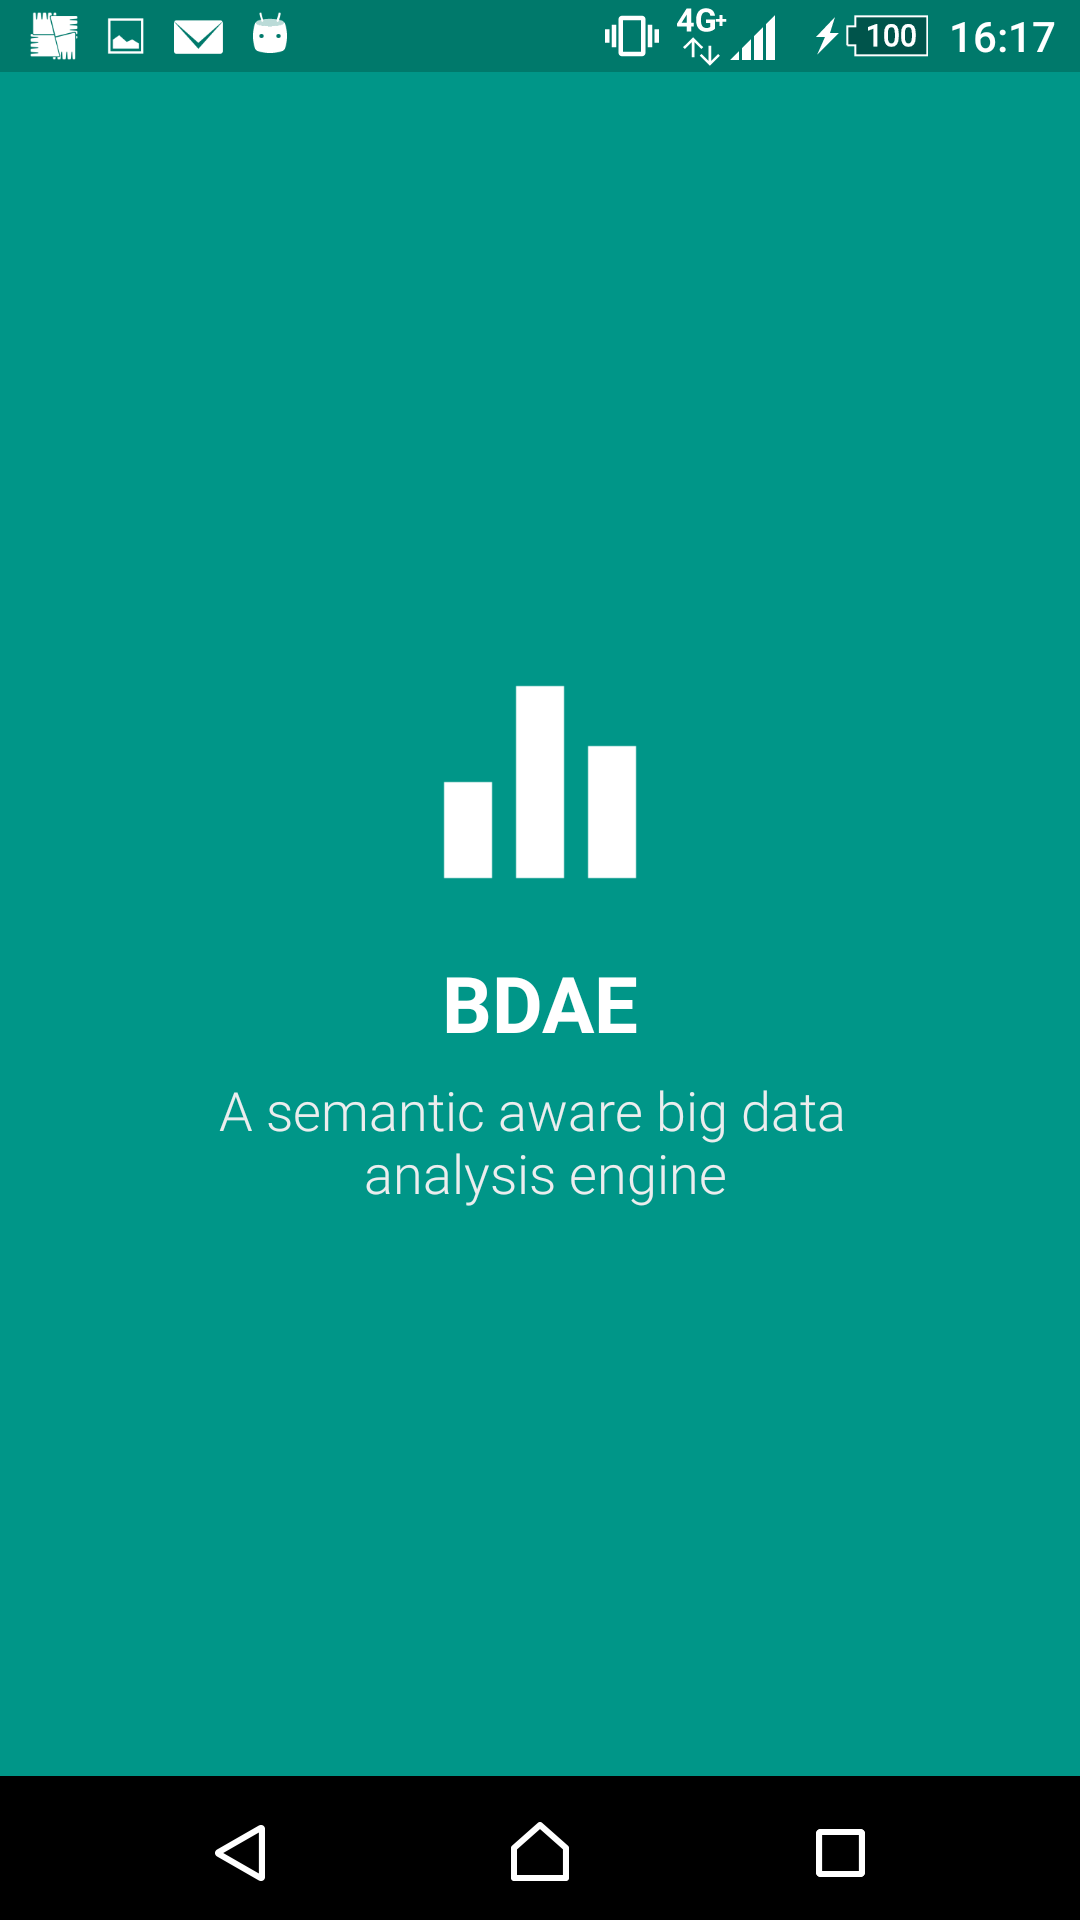
\includegraphics[width=\textwidth]{img/loadingscreen.png}
    \end{minipage}
  	\hfill
  	\begin{minipage}[b]{0.4\textwidth}
    		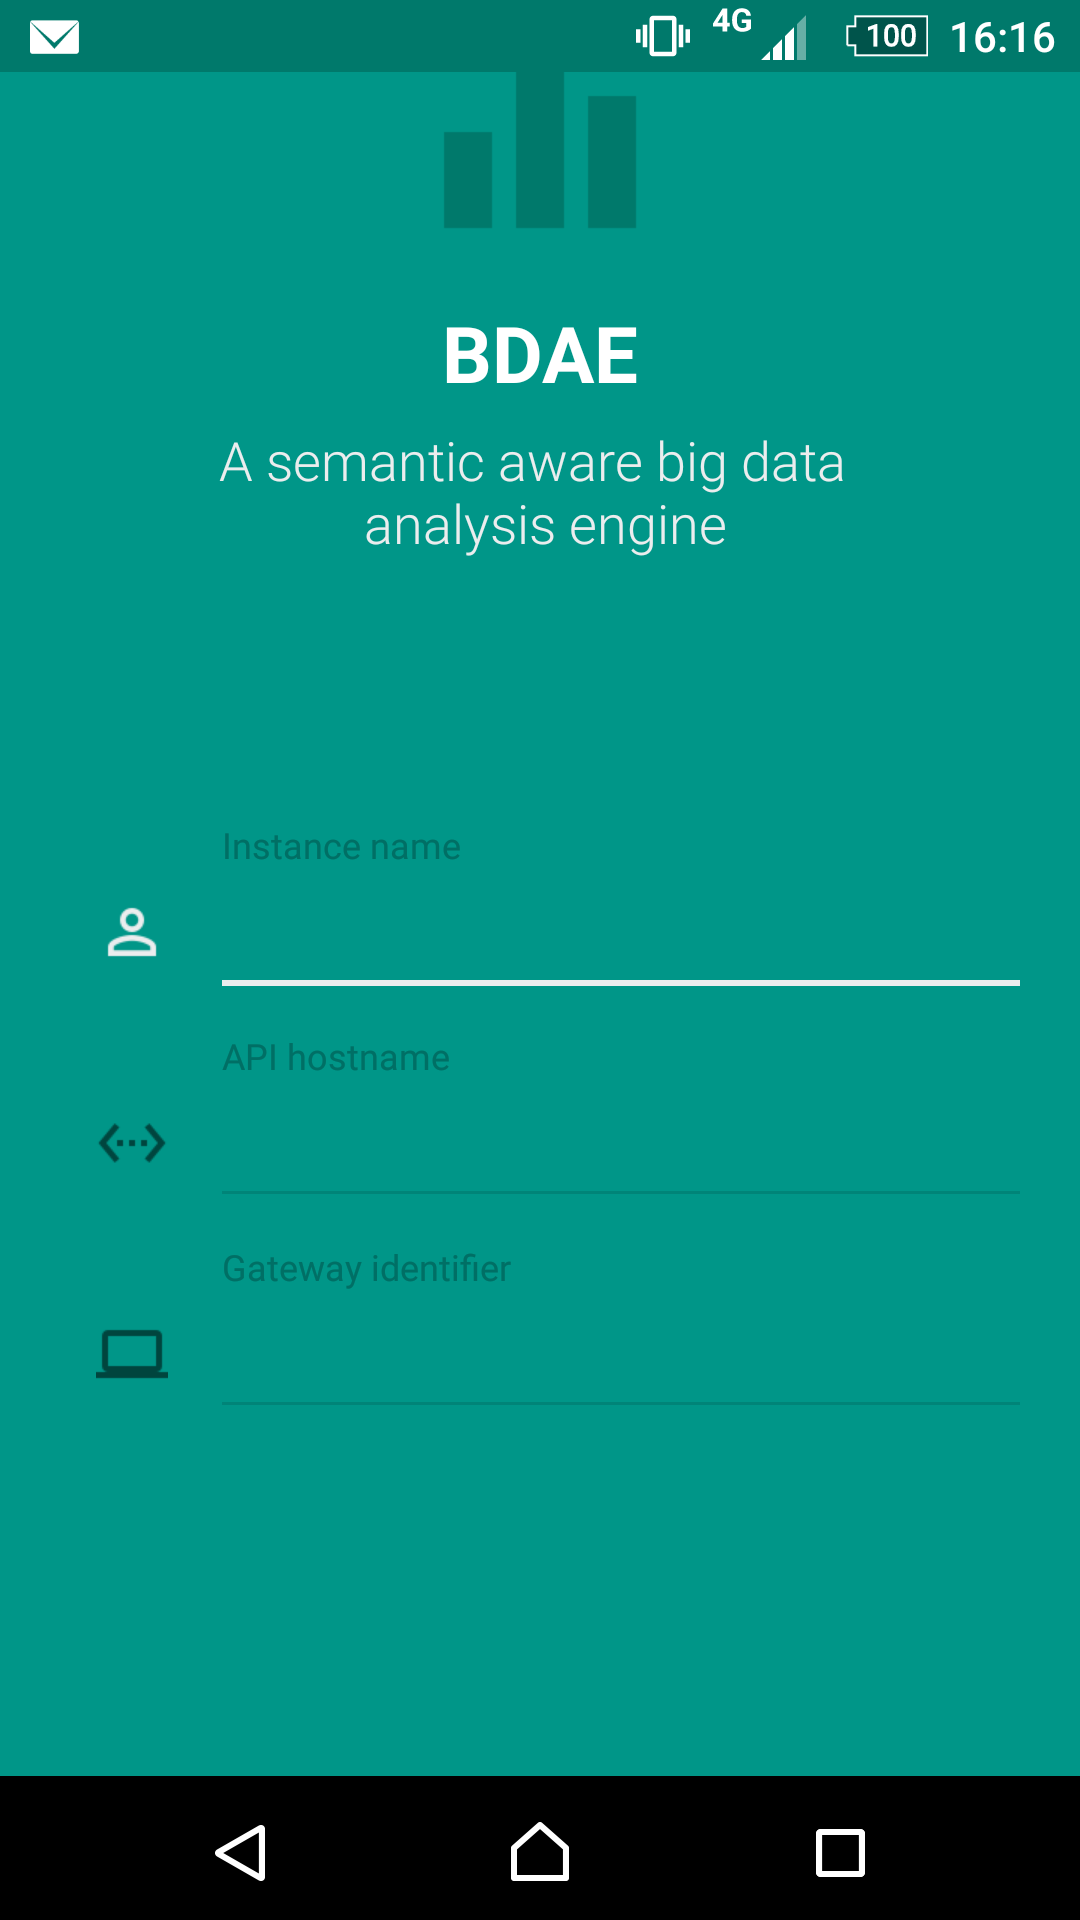
\includegraphics[width=\textwidth]{img/information.png}
  	\end{minipage}
  	\caption[]{Loading screen animated into the required information screen.}
\end{figure*}

\begin{figure*}[h!]
	\centering
  	\begin{minipage}[b]{0.4\textwidth}
    		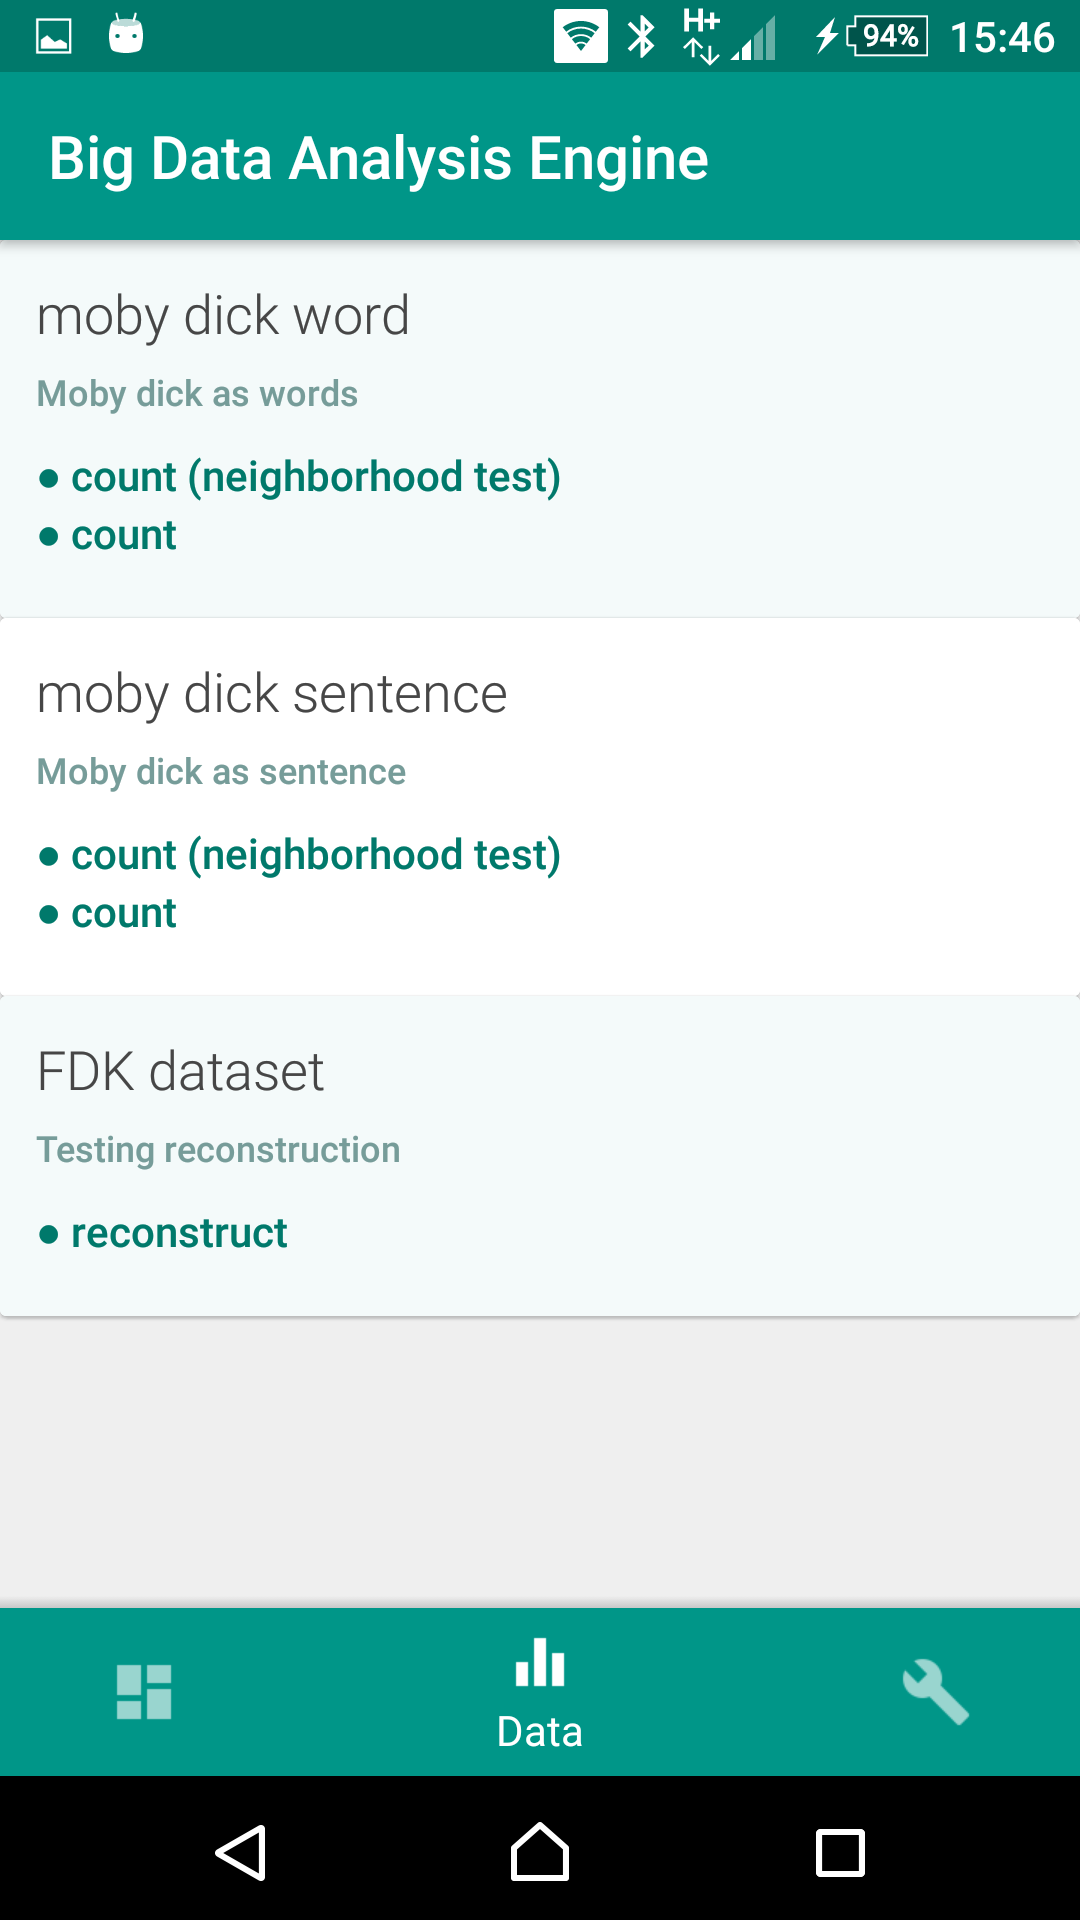
\includegraphics[width=\textwidth]{img/datasets.png}
   	  	\caption[]{List of available datasets and their associated operations.}
    \end{minipage}
  	\hfill
  	\begin{minipage}[b]{0.4\textwidth}
    		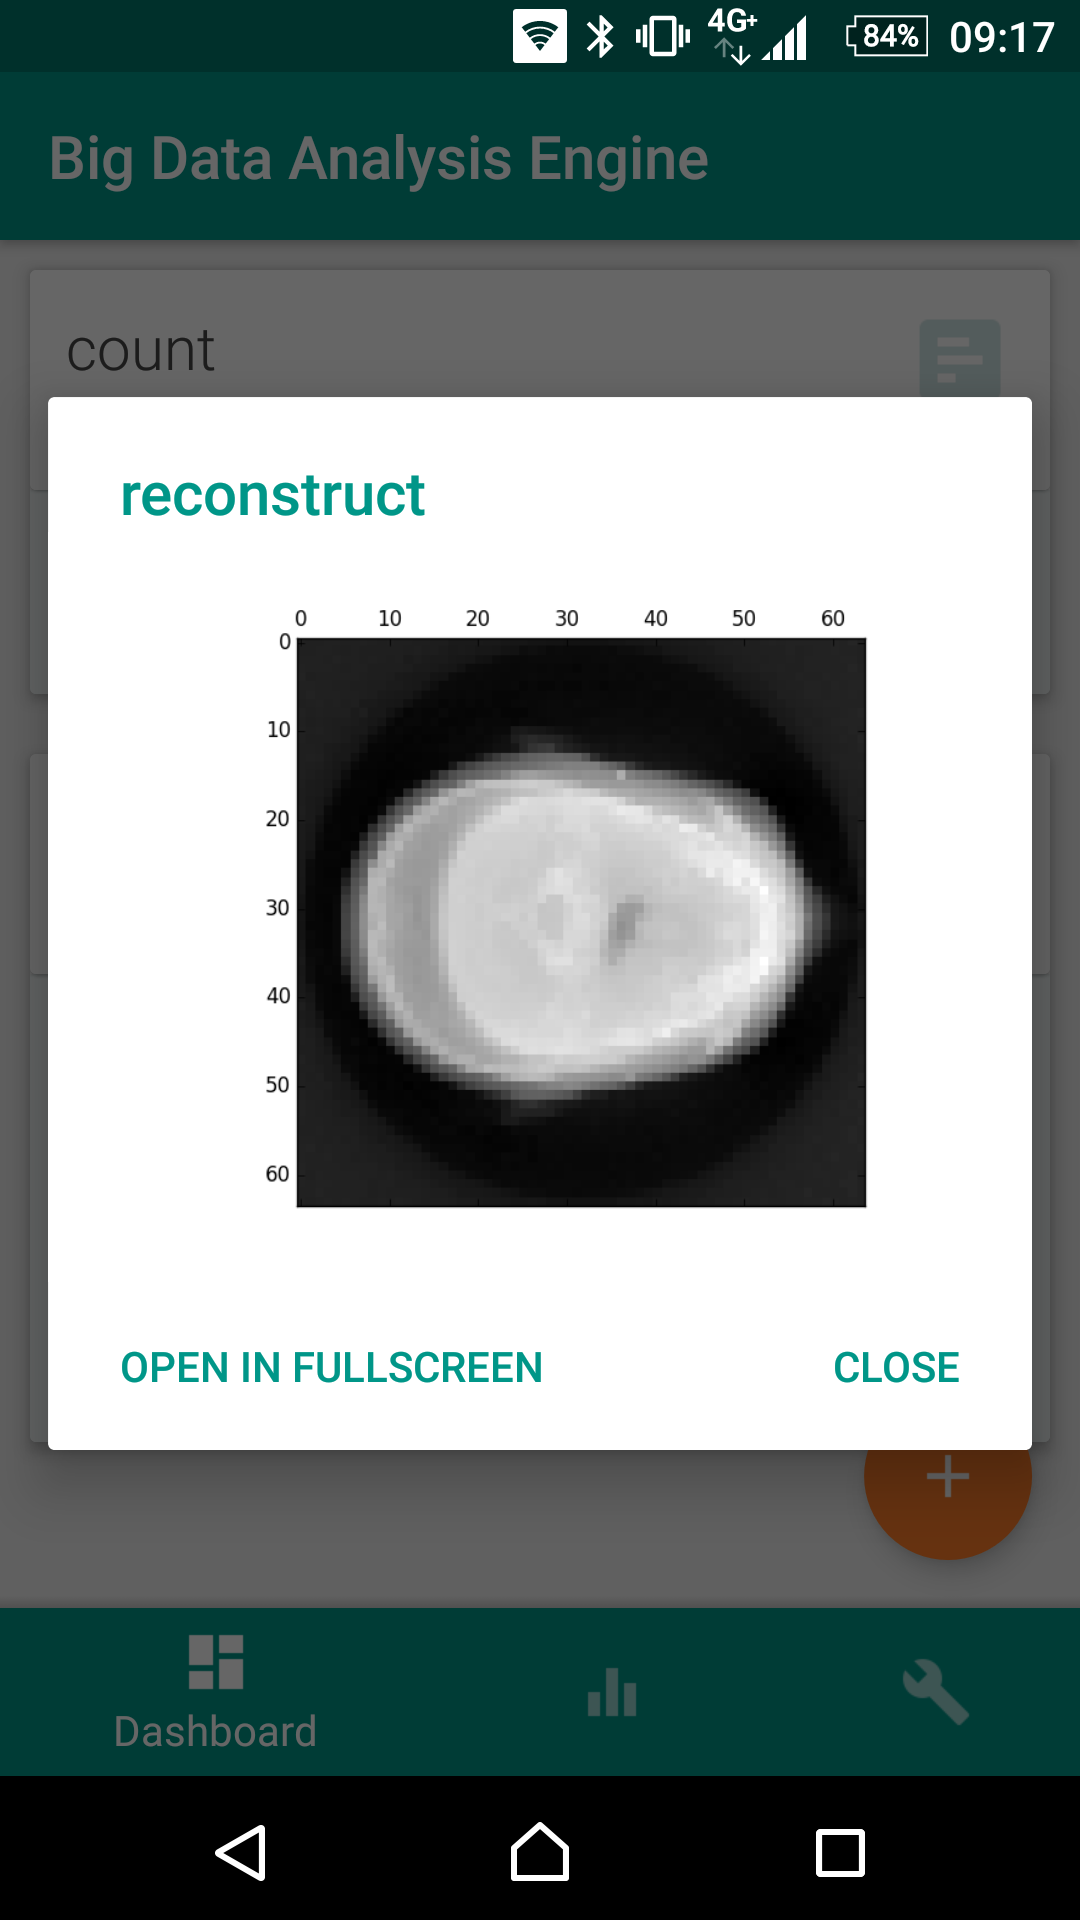
\includegraphics[width=\textwidth]{img/result.png}
    		\caption[]{A dialog displaying the result of a CT reconstruction operation.}
  	\end{minipage}
\end{figure*}

\chapter{Benchmark Graphs}
\section{CT reconstruction} \label{app:fdk}
\begin{figure}[h!]
	\centering
	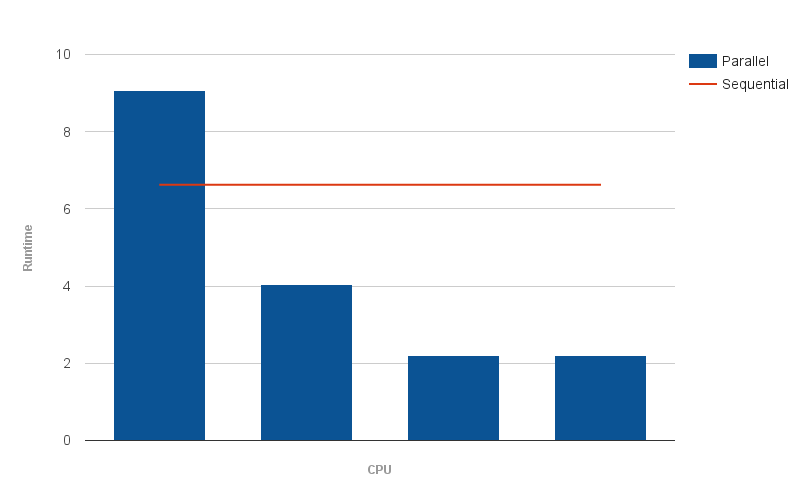
\includegraphics[scale=0.4]{img/fdk-64.png}
	\caption[]{Execution time of the 64x64x64 voxels dataset. \label{fig:fdk-64}}
\end{figure}

\begin{figure}[h!]
	\centering
	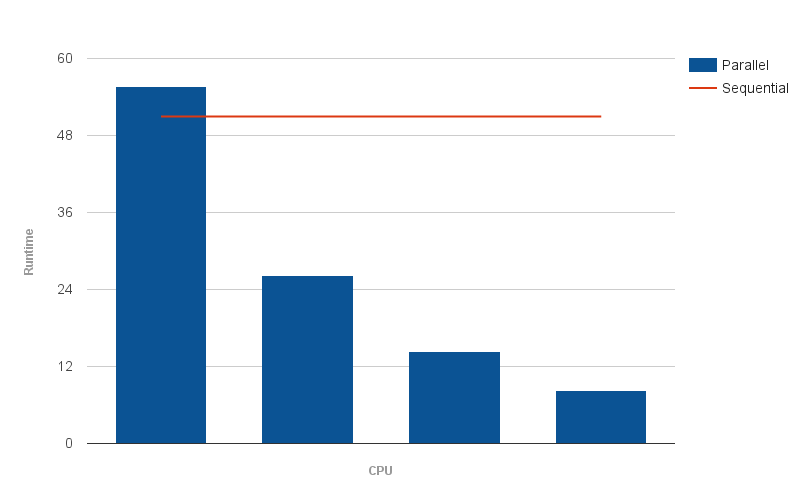
\includegraphics[scale=0.4]{img/fdk-128.png}
	\caption[]{Execution time of the 128x128x128 voxels dataset. \label{fig:fdk-128}}
\end{figure}

\begin{figure}[h!]
	\centering
	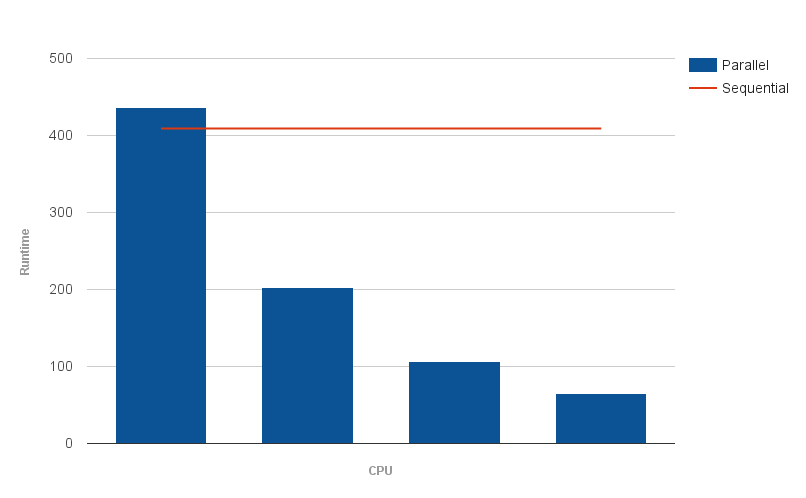
\includegraphics[scale=0.4]{img/fdk-256.png}
	\caption[]{Execution time of the 256x256x256 voxels dataset. \label{fig:fdk-256}}
\end{figure}

\chapter{Hadoop Source Code Example}
\definecolor{pblue}{rgb}{0.13,0.13,1}
\definecolor{pgreen}{rgb}{0,0.5,0}
\definecolor{pred}{rgb}{0.9,0,0}
\definecolor{pgrey}{rgb}{0.46,0.45,0.48}

\section{Map} \label{sec:hadoop-map}
\begin{lstlisting}[language=Java, commentstyle=\color{pgreen}, keywordstyle=\color{pblue}, stringstyle=\color{pred},basicstyle=\fontsize{6}{5}\selectfont\ttfamily, xleftmargin=0.8cm]
package com.cloudera.example;

import org.apache.hadoop.io.IntWritable;
import org.apache.hadoop.io.LongWritable;
import org.apache.hadoop.io.Text;
import org.apache.hadoop.mapreduce.Mapper;

import java.io.IOException;

public class LogEventParseMapper extends Mapper<LongWritable, Text, Text, IntWritable> {
    
    enum Level { TRACE, DEBUG, INFO, WARN, ERROR, FATAL };

    @Override
    public void map(LongWritable key, Text value, Context context)
            throws IOException, InterruptedException {

        String line = value.toString();

        // ignore empty lines
        if (line.trim().isEmpty()) {
            return;
        }
        String[] fields = line.split(" ");

        // ensure this line is not malformed
        if (fields.length <= 3) {
            return;
        }

        String levelField = fields[3];
        for (Level level : Level.values()) {
            String levelName = level.name();
            if (levelName.equalsIgnoreCase(levelField)) {
                context.write(new Text(levelName), new IntWritable(1));
            }
        }
    }
}
\end{lstlisting}
\newpage
\section{Reduce} \label{sec:hadoop-reduce}
\begin{lstlisting}[language=Java, commentstyle=\color{pgreen}, keywordstyle=\color{pblue}, stringstyle=\color{pred},basicstyle=\fontsize{6}{5}\selectfont\ttfamily, xleftmargin=0.8cm]
package com.cloudera.example;

import java.io.IOException;

import org.apache.hadoop.io.IntWritable;
import org.apache.hadoop.io.Text;
import org.apache.hadoop.mapreduce.Reducer;

public class LogEventSumReducer extends Reducer<Text, IntWritable, Text, IntWritable> {

    @Override
    public void reduce(Text key, Iterable<IntWritable> values, Context context) 
            throws IOException, InterruptedException {

        // used to count the number of messages for this event type
        int sum = 0;
        // increment it for each new value received
        for (IntWritable value : values) {
            sum += value.get();
        }

        // Our output is the event type (key) and the sum (value)
        context.write(key, new IntWritable(sum));
    }
}
\end{lstlisting}

\backmatter
\renewcommand*{\printchaptertitle}[1]{\flushleft\chaptitlefont#1}
\renewcommand*{\chaptitlefont}{\normalfont\sffamily\Huge\bfseries}
\chaptermark{Bibliography}
\renewcommand{\sectionmark}[1]{\markright{#1}}
\sectionmark{Bibliography}
\bibliographystyle{ieeetr}
\bibliography{tex/references}

\end{document}